\documentclass[12pt]{article}

% Package for page layout
\usepackage[margin=1in]{geometry}
\usepackage{amsmath}
\usepackage{amssymb}
\usepackage{algorithm}
\usepackage{algpseudocode}
\usepackage{forest}
\usepackage{adjustbox}
\definecolor{lightred}{RGB}{255, 204, 203}
\definecolor{lightgreen}{RGB}{197, 224, 180}
\definecolor{lightyellow}{RGB}{255, 255, 153}

% Package for double spacing
\usepackage{setspace}
\doublespacing
\setlength{\parskip}{\baselineskip} % Sets paragraph separation to one base line skip

% Package for images
\usepackage{graphicx}

% Package for bibliography
\usepackage[backend=bibtex,style=numeric,sorting=none]{biblatex}
\addbibresource{references.bib} % Your bibliography file

% Package for tables
\usepackage{tabularx}

\begin{document}

\title{Comprehensive survey on Diffusion Models: From Image generation to 3D NeRF Generation}
\author{Naman Garg\\
\small Northwestern University\\
\small \texttt{namangarg2025@u.northwestern.edu}}
\date{March 1, 2024}
\maketitle

\begin{abstract}
This survey paper provides an in-depth exploration of diffusion models, 
tracing their evolution from theoretical concepts in thermodynamics to their
essential role in modern machine learning and artificial intelligence. 
It highlights key technological advancements that have established diffusion 
models as leading tools for generating high-quality, diverse images, videos,
and more, while also adapting to various types of conditioning data. The paper 
covers a broad range of applications, from traditional image and video 
processing to innovative uses in 3D model creation and document layout
generation. It addresses the significant challenges faced by diffusion models
, such as computational demands and the generation accuracy relative to complex
text prompts, and proposes potential solutions and future research directions 
to overcome these obstacles. By offering a comprehensive review and insightful 
analysis, this survey aims to serve as a valuable resource for both researchers and practitioners,
guiding further advancements and innovation in the field of diffusion models.
\end{abstract}

\section{Introduction}
Image generation has long been at the forefront of research in computer vision and artificial intelligence. From the initial forays with Variational Autoencoders (VAEs) \cite{Kingma2013} and Generative Adversarial Networks (GANs) \cite{Goodfellow2014} to the recent breakthroughs in photorealistic image synthesis, the field has seen rapid evolution. VAEs, which are neural networks designed to encode and decode images, laid the groundwork for understanding complex data distributions. GANs, comprising two competing networks, further advanced the capability to generate new, high-quality images by learning to mimic the distribution of real images.

Diffusion models have disrupte the longstanding dominance of GANs \cite{Goodfellow2014} and VAEs \cite{Kingma2013} in the realm of image generation. These novel generative models are currently receiving significant attention. Originating from the domain of thermodynamics, the concept of diffusion models introduces a fresh approach to image generation \cite{Sohl-Dickstein2015}. The underlying idea posits that gradually introducing noise into an image until it is completely transformed into noise—and then reversing this process—mirrors the core principles of generating images. This reversal process, if successfully learned by deep learning techniques, could revolutionize image generation. Further, the mathematical foundation of diffusion models was solidified with the use of Markov chains in Denoising Diffusion Probabilistic Models (DDPM) \cite{DDPM}, providing a robust theoretical framework that enhances our understanding and capabilities in generating complex images.

The advent of open-source initiatives like Stability.ai's Stable Diffusion marked a significant leap forward. These models have democratized access to advanced image generation technologies, catalyzing both academic research and product innovation. Unlike their predecessors, diffusion models generate images through a process of gradually refining random noise, aligning more closely with how humans might imagine and create images from scratch \cite{LDM}.

Recently, these models have been enhanced by training on image-caption pairs, leveraging techniques such as those introduced by CLIP (Contrastive Language–Image Pre-training) to align images with text prompts more effectively \cite{CLIP}. To navigate away from the adversarial nature of GANs, Classifier-Free Guidance (CFG) emerged as a method to improve the fidelity and diversity of generated images without the need for a discriminator network \cite{CFG}.

Despite these advancements, the quest for models that can faithfully adhere to all elements of a text prompt remains ongoing. The gap between the complexity of human language and the interpretative capability of AI models poses a significant challenge. Innovations like ControlNet offer a promising direction by incorporating additional inputs such as depth maps and pose maps to provide nuanced control over the image generation process \cite{ControlNet}. However, achieving perfect alignment between text prompts and generated images is still a complex challenge that the field continues to grapple with.

Moreover, these image generation models still struggle with finer details, such as accurately generating text within images or getting the right number of fingers on a hand. These seemingly minor inaccuracies highlight the ongoing challenges in creating truly lifelike and accurate images.

The application of diffusion models extends beyond mere image creation; they have been successfully applied to image editing, video generation and editing, 3D model generation from text or images, and even document layout generation. This survey paper aims to delve into the multifaceted world of diffusion models, exploring their components, evolutionary trajectory, limitations, and the ingenious solutions devised to overcome these hurdles.

A comprehensive mindmap detailing the development and evolution of diffusion models is included in Figure 1. This visual representation provides an overview of the key milestones, technologies, and innovations that have shaped the current landscape of diffusion models.

As we chart the course of diffusion models from their inception to their current state, and look towards the future, it becomes evident that while significant strides have been made, the journey is far from over. The potential for further breakthroughs and applications is vast, promising a dynamic and exciting future for image generation technology.


\begin{figure}[]
    \centering
    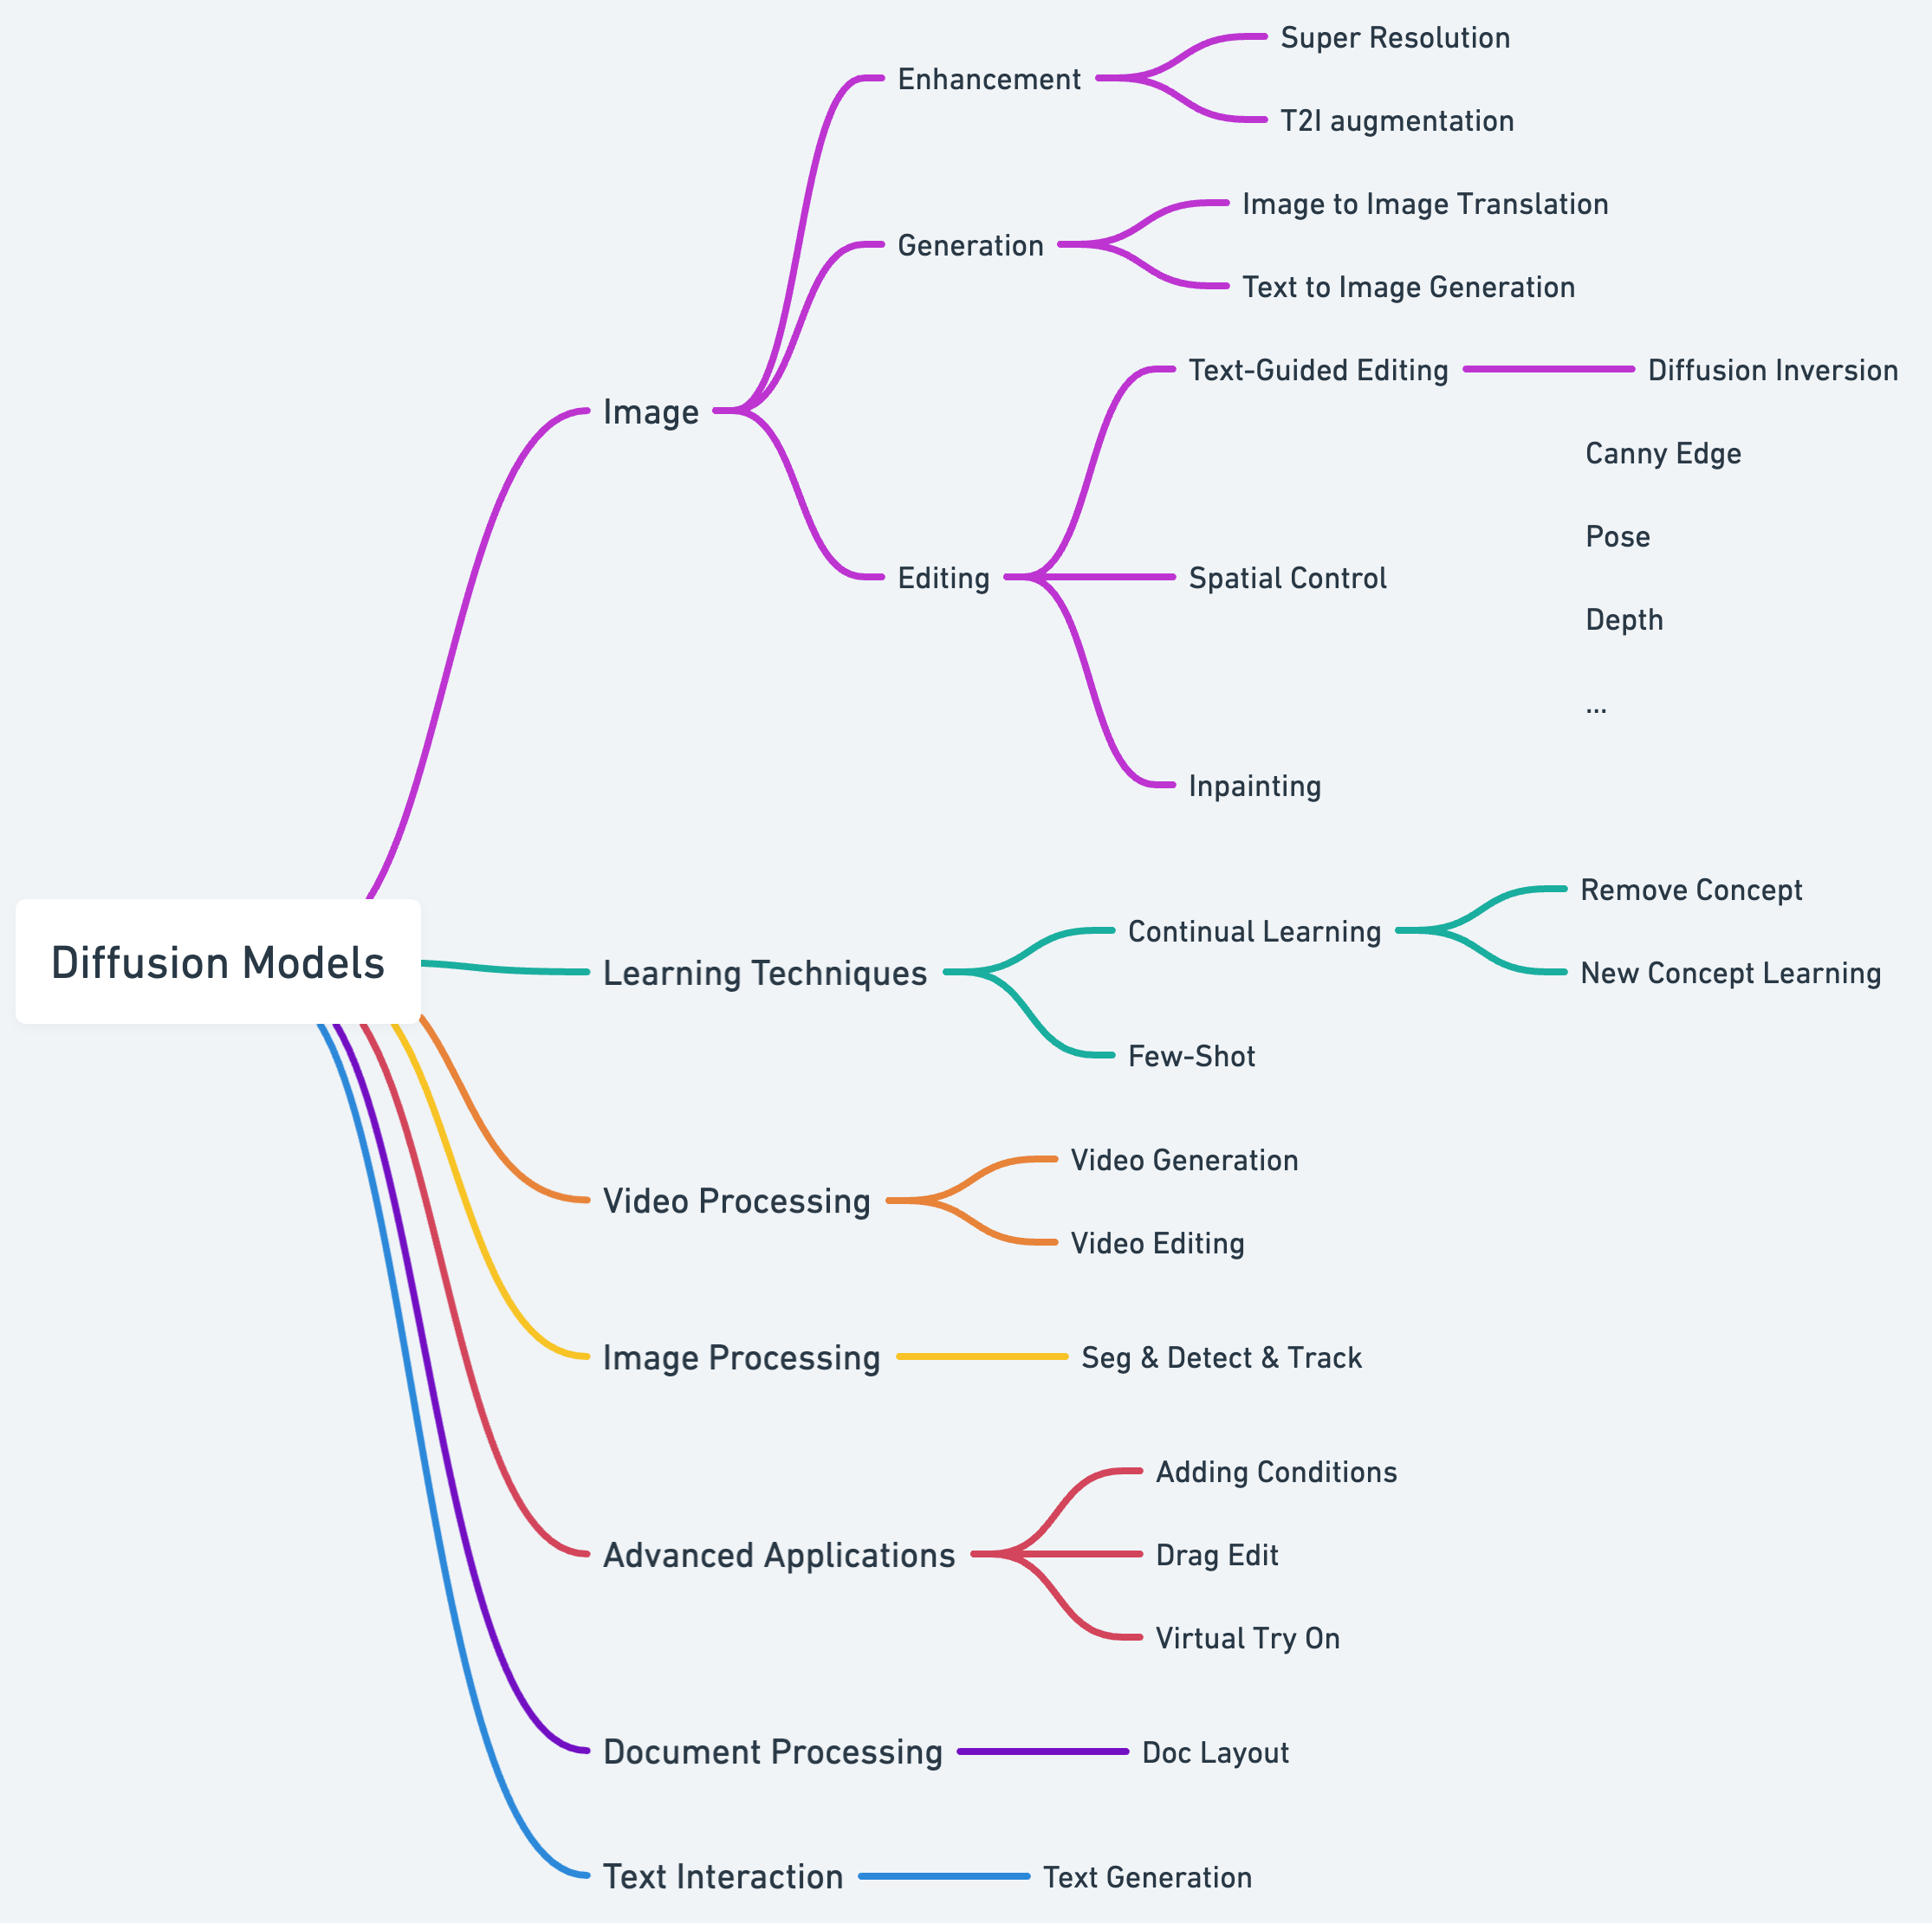
\includegraphics[width=\textwidth]{images/mind-map.png}
    \caption{Mind Map of diffusion models}
    \end{figure}

\section{PRELIMINARIES OF DIFFUSION MODELS}
Image Diffusion Models were first introduced by SohlDickstein et al. 
\cite*{Sohl-Dickstein2015,kingma2021variational} and have been recently applied to
image generation \cite*{dhariwal2021diffusion,}. The Latent Diffusion Models
(LDM) \cite*{LDM} performs the diffusion steps in the latent image
space [19], which reduces the computation cost. Text-toimage diffusion models achieve state-of-the-art image generation results by encoding text inputs into latent vectors
via pretrained language models like CLIP \cite*{CLIP}. Glide \cite*{glide}
is a text-guided diffusion model supporting image generation and editing. Disco Diffusion [5] processes text prompts
with clip guidance. Stable Diffusion \cite*{stablediffusionv15} is a large-scale
implementation of latent diffusion \cite*{LDM}. Imagen \cite*{saharia2022photorealistic} directly
diffuses pixels using a pyramid structure without using latent
images. Commercial products include DALL-E2 \cite*{openai2023dalle2} and
Midjourney \cite*{midjourney2023}.




\subsection{Exploration of Denoising Diffusion Probabilistic Models}

Denoising Diffusion Probabilistic Models (DDPMs) \cite*{DDPM} introduce an innovative framework for generative models that emphasize the reverse engineering of diffusion processes. These models utilize parameterized Markov chains to methodically transform noise into organized patterns over multiple iterations.

The diffusion phase commences with an initial distribution \(x_0 \sim q(x_0)\), methodically incorporating Gaussian noise over \(T\) timesteps. At each step \(t\), the noising process is characterized by:
\begin{equation}
q(x_{1:T}|x_0) = \prod_{t=1}^{T} q(x_t|x_{t-1}),
\end{equation}

\begin{equation}
q(x_t|x_{t-1}) = \mathcal{N}(x_t; \sqrt{1-\beta_t}x_{t-1}, \beta_t\mathbf{I}),
\end{equation}
where \( \beta_t \) represents the stepwise noise variance parameters.

In the denoising phase, DDPMs aim to incrementally cleanse the data, effectively reversing the diffusion sequence. This begins from a noisy state \(x_T\) and progressively works towards the initial data distribution \(q(x_0)\). The model specifies the reverse transition \(p_{\theta}(x_{t-1}|x_t)\) with:
\begin{equation}
p_{\theta}(x_{t-1}|x_t) = \mathcal{N}(x_{t-1}; \mu_{\theta}(x_t, t), \Sigma_{\theta}(x_t, t))
\end{equation}
Deep learning models, notably those based on UNet architectures, parameterize \( \mu_{\theta}(x_t, t) \) and \( \Sigma_{\theta}(x_t, t) \). These models input the noised data \(x_t\) and timestep \(t\), predicting the normal distribution's parameters to identify the noise \( \epsilon_{\theta} \) needed for reversing the diffusion. Generating new data instances \(x_0\) involves starting with a noise vector \(x_T \sim p(x_T)\) and sequentially sampling from \(p_{\theta}(x_{t-1}|x_t)\) until \(t=1\), completing the reverse diffusion pathway.

The methodologies underlying the training and sampling of DDPMs are elucidated through pseudocode in the referenced Algorithm \ref{alg:ddpm_training} and Algorithm \ref{alg:ddpm_sampling}. These algorithms detail the procedural steps for both learning the model parameters and generating new samples, providing a comprehensive understanding of the operational framework of DDPMs.


\begin{algorithm}
    \caption{DDPM Training}\label{alg:ddpm_training}
    \begin{algorithmic}[1]
    \Repeat
        \State $x_0 \sim q(x_0)$
        \State $t \sim \text{Uniform}\{1, \ldots, T\}$
        \State $\varepsilon \sim \mathcal{N}(0, I)$
        \State Take gradient descent step on
        \State $\nabla_\theta \left\| \varepsilon - \varepsilon_\theta(\sqrt{\alpha_t}x_0 + \sqrt{1 - \alpha_t} \varepsilon, t) \right\|^2$
    \Until{converged}
    \end{algorithmic}
    \end{algorithm}
    
\begin{algorithm}
    \caption{DDPM Sampling}\label{alg:ddpm_sampling}
    \begin{algorithmic}[1]
    \State $x_T \sim \mathcal{N}(0, I)$
    \For{$t = T, \ldots, 1$}
        \State $z \sim \begin{cases} 
        \mathcal{N}(0, I) & \text{if } t > 1 \\
        0 & \text{else}
        \end{cases}$
        \State $x_{t-1} = \frac{1}{\sqrt{\alpha_t}} \left(x_t - \frac{1-\alpha_t}{\sqrt{1 - \alpha_t}} \varepsilon_\theta(x_t, t)\right) + \sigma_t z$
    \EndFor
    \State \Return $x_0$
    \end{algorithmic}
    \end{algorithm}

\begin{figure}[h!]
    \centering
    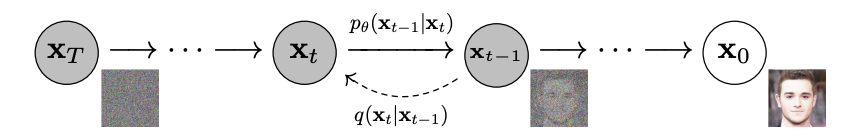
\includegraphics[width=\textwidth]{images/DDPM.png}
    \caption{Mind Map of diffusion models \cite*{DDPM}}
\end{figure}




\section{Guiderails for Constrained Generation}
Diffusion models have emerged as a powerful class of generative models, enabling the generation of high-quality, diverse samples across various domains, including images, text, and audio. To direct the generation process towards desired outcomes, various guiderail mechanisms have been developed, including explicit conditioning, classifier guidance, and classifier-free guidance. These mechanisms constrain the generative process, ensuring that the output adheres to specific criteria or characteristics, thereby enhancing the model's utility for practical applications.

\subsection{Explicit Conditioning}
Explicit conditioning involves providing the diffusion model with additional context or information, guiding the generation process towards a specific outcome. This can be in the form of textual descriptions, labels, or any form of metadata that describes the desired output characteristics. For instance, in image generation, a text description can serve as a condition to generate images that match the described content. The effectiveness of explicit conditioning lies in its ability to leverage the conditional distribution learned by the model to produce outputs that closely align with the provided context or information.

\subsection{Classifier Guidance}
Classifier guidance integrates a separate classifier model to steer the generation process of the diffusion model. The classifier is trained to distinguish between desirable and undesirable outputs based on predefined criteria. During generation, the gradient signals from the classifier are used to adjust the diffusion process, pushing the generated samples towards the characteristics identified as desirable. This method allows for fine-grained control over the generation process, enabling the production of outputs that meet specific quality or content standards.

\subsection{Classifier-Free Guidance}
Classifier-free guidance is a technique that eliminates the need for a separate classifier model. Instead, it leverages the inherent capability of the diffusion model to differentiate between various outcomes. This is achieved by intermittently conditioning the model on a null input (i.e., providing no specific guidance) and comparing the output against those generated with explicit conditioning. The difference in outputs guides the adjustment of the generation process, encouraging the model to produce samples that are more closely aligned with the desired conditions, even in the absence of a dedicated classifier. This approach simplifies the generation process, reducing the computational overhead and complexity associated with maintaining a separate classifier model. \cite*{CFG}

\subsection{Some other methods}
Each of these guidance mechanisms serves to constrain and direct the generation process of diffusion models, enabling the creation of outputs that meet specific criteria or exhibit desired characteristics. The choice of mechanism depends on the specific requirements of the application, including the level of control needed, the availability of conditional information, and computational constraints.


The ability to steer image diffusion models enhances personalization, customization, and task-specific image generation. Direct manipulation of the image diffusion process enables adjustments in color variations \cite{sdedit2021} and facilitates inpainting tasks \cite{blended2022}. Text-guided controls extend these capabilities through prompt modification, CLIP feature manipulation, and cross-attention adjustments \cite{makeascene2022, spatext2022, gligen2023, textualinversion2022, dreambooth2022, promptedit2022}. Techniques like encoding segmentation masks into tokens for image generation control in MakeAScene \cite{makeascene2022}, or mapping these masks into localized token embeddings in SpaText \cite{spatext2022}, showcase the diversity of approaches. GLIGEN \cite{gligen2023} introduces parameter adjustments in attention layers for more grounded generation processes. Personalization is further achieved through methods like Textual Inversion \cite{textualinversion2022} and DreamBooth \cite{dreambooth}, which fine-tune diffusion models using a collection of user-provided example images. Prompt-based editing methods \cite{promptedit2022} offer practical solutions for image manipulation. Furthermore, optimization techniques that align the diffusion process with sketches have been proposed \cite{sketchdiffusion2022}, alongside studies like MultiDiffusion \cite{multidiffusion2023}, which explore various control strategies over diffusion models.

\subsection{ControlNet}

\cite*{ControlNet} presents ControlNet, a novel neural network architecture designed to incorporate spatial conditioning controls into large pre-trained text-to-image diffusion models. ControlNet leverages the depth and robustness of the encoding layers from these pre-trained models, providing a powerful backbone for learning a variety of conditional controls. By employing "zero convolutions," which are convolution layers initialized with zeros, ControlNet ensures a seamless and noise-free integration of conditions into the diffusion process. This architecture allows for the manipulation of images using various conditions, such as edges, depth, segmentation, and human pose, with or without accompanying text prompts. The experiments demonstrate that ControlNet can effectively handle single or multiple conditions and is robust across different dataset sizes. It offers significant advancements in controlled image generation, potentially broadening the application scope of diffusion models in image editing, content creation, and beyond.








\definecolor{hidden-draw}{RGB}{161,165,193}
\definecolor{hidden-pink}{RGB}{244,243,250}
\begin{figure}[H]
    \centering
    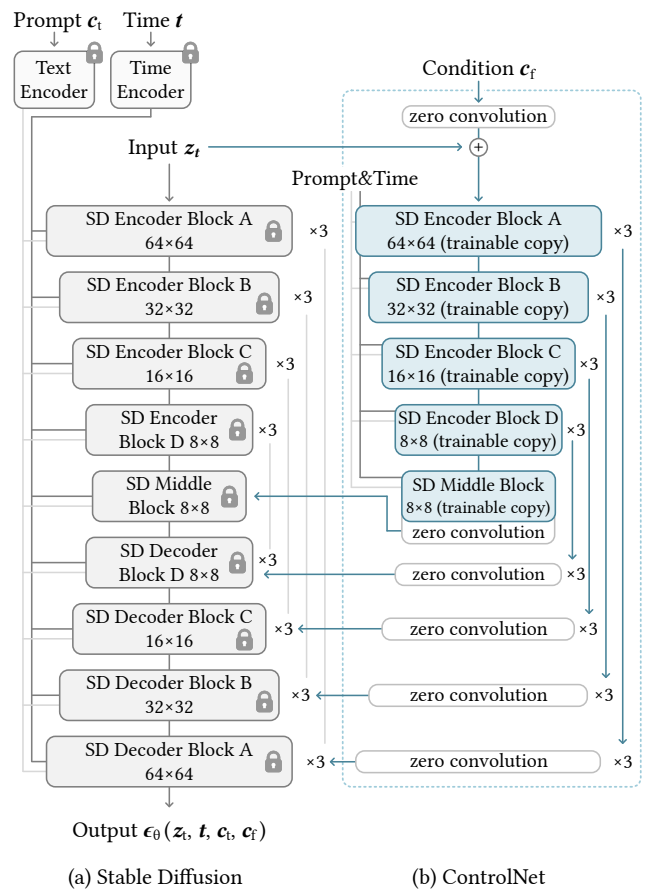
\includegraphics[width=0.60\textwidth]{images/controlnet.png} % Adjust the width as needed
    \caption{ControlNet: Guiding model through Canny, Depth Map, Pose Map, etc. \cite*{ControlNet}}
\end{figure}


\begin{figure}[H]
    \centering
    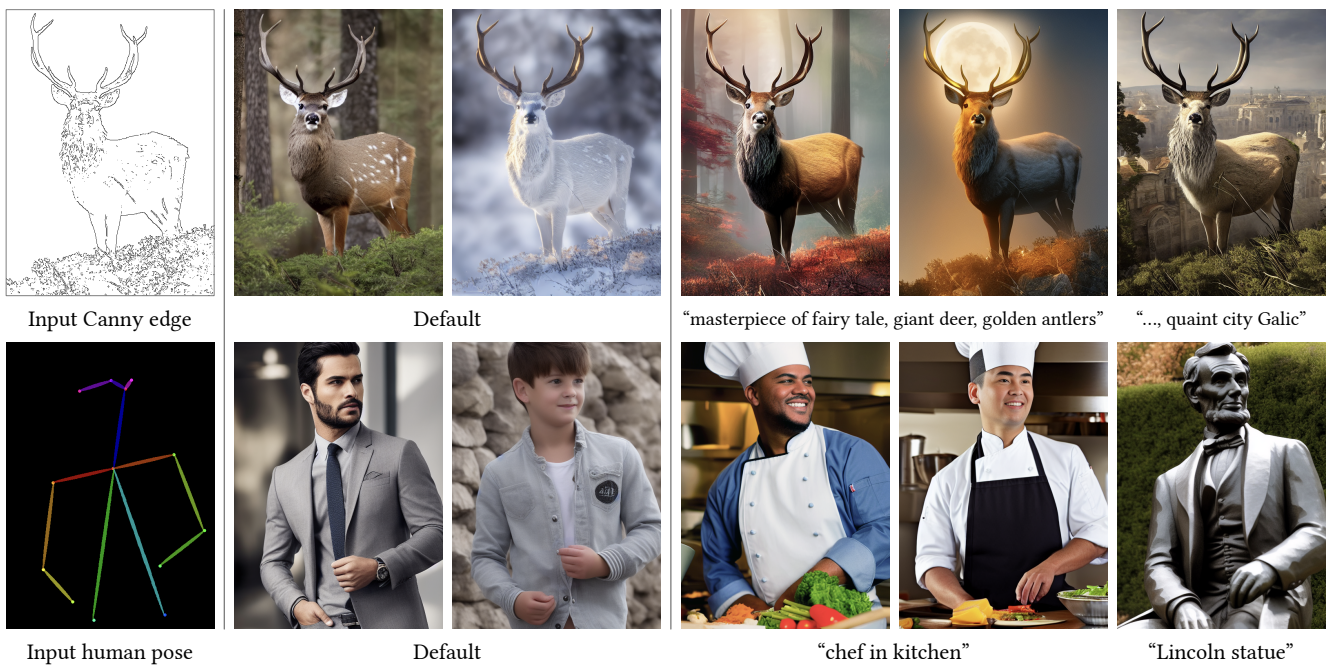
\includegraphics[width=1\textwidth]{images/controlnet_result.png}
    \caption{Controlling Stable Diffusion with learned conditions. ControlNet allows users to add conditions like Canny edges
    (top), human pose (bottom), etc., to control the image generation of large pretrained diffusion models. The default results use
    the prompt “a high-quality, detailed, and professional image”. Users can optionally give prompts like the “chef in kitchen”. \cite*{ControlNet}}
\end{figure}


% \tikzstyle{my-box}=[
%     rectangle,
%     draw=hidden-draw,
%     rounded corners,
%     text opacity=1,
%     minimum height=1.5em,
%     minimum width=5em,
%     inner sep=2pt,
%     align=center,
%     fill opacity=.5,
%     line width=0.8pt,
% ]
% \tikzstyle{leaf}=[my-box, minimum height=1.5em,
%     fill=hidden-pink!80, text=black, align=left,font=\tiny,
%     inner xsep=2pt,
%     inner ysep=4pt,
%     line width=0.8pt,
% ]


% \begin{figure*}[t!]
%     \centering
%     \resizebox{0.5\textwidth}{!}{
%         \begin{forest}
%             forked edges,
%             for tree={
%                 grow=east,
%                 reversed=true,
%                 anchor=base west,
%                 parent anchor=east,
%                 child anchor=west,
%                 base=left,
%                 font=\tiny,
%                 rectangle,
%                 draw=hidden-draw,
%                 rounded corners,
%                 align=left,
%                 minimum width=2em,
%                 edge+={darkgray, line width=1pt},
%                 s sep=3pt,
%                 inner xsep=2pt,
%                 inner ysep=3pt,
%                 line width=0.8pt,
%                 ver/.style={rotate=90, child anchor=north, parent anchor=south, anchor=center},
%             },
%             where level=1{text width=6em,font=\tiny,}{},
%             where level=2{text width=4.3em,font=\tiny,}{},
%             where level=3{text width=4.0em,font=\tiny,}{},
%             [
%                 Controllable Generation with Text-to-Image Diffusion Models, ver
%                 [
%                     Generation with \\ specific condition (\S \ref{sec:method})
%                     [
%                         Personalization \\ (\S~\ref{sec:personalization})
%                         [
%                            \textbf{(a) Subject-Driven:} Textual Inversion\cite{gal2022image} {,} Dreambooth\cite{ruiz2023dreambooth} {,} Re-Imagen\cite{chen2022re} {,} DreamArtist\cite{dong2022dreamartist} {,} \\Custom Diffusion\cite{kumari2023multi} {,} DVAR\cite{voronov2023loss} {,} E4T\cite{gal2023designing} {,} ELITE\cite{wei2023elite} {,} UMM-Diffusion\cite{ma2023unified} {,} XTI\cite{voynov2023p+} {,} SVDiff\cite{han2023svdiff} {,} \\ANOVA\cite{xiang2023closer} {,} SuTI\cite{chen2023subject} {,} Jia \emph{et al.}\cite{jia2023taming} {,} InstantBooth\cite{shi2023instantbooth} {,} COTI\cite{yang2023controllable} {,} Gradient-Free TI\cite{fei2023gradient} {,} Perfusion\cite{tewel2023key} {,} \\DisenBooth\cite{chen2023disenbooth} {,} BLIP-Diffusion\cite{li2023blip} {,} ProSpect\cite{zhang2023prospect} {,} Break-A-Scene\cite{avrahami2023break} {,} COMCAT\cite{xiao2023comcat} {,} OFT\cite{qiu2023controlling} {,} \\PACGen\cite{li2023generate} {,} Arar \etal\cite{arar2023domain} {,} Subject-Diffusion\cite{ma2023subject} {,} LyCORIS\cite{yeh2023navigating} {,} Kosmmos-G\cite{pan2023kosmos} {,} MCPL\cite{jin2023image} {,} \\He \emph{et al.}\cite{he2023data} {,} KC Loss\cite{roy2023diffnat} {,} MATTE\cite{agarwal2023image} {,} Lego\cite{motamed2023lego} {,} CatVersion\cite{zhao2023catversion} {,} CLiC\cite{safaee2023clic} {,} VideoAssembler\cite{zhao2023videoassembler} {,} \\ HiFi Tuner\cite{wang2023hifi} {,} VideoBooth\cite{jiang2023videobooth} {,} CAFE\cite{zhou2023customization} {,} DETEX\cite{cai2023decoupled} {,} DreamTuner\cite{hua2023dreamtuner} \\
% 							\textbf{(b) Person-Driven:} FastComposer\cite{xiao2023fastcomposer} {,} Giambi \emph{et al.}\cite{giambi2023conditioning} {,} Face0\cite{valevski2023face0} {,} DreamIdentity\cite{chen2023dreamidentity} {,}\\ HyperDreamBooth\cite{ruiz2023hyperdreambooth} {,} PhotoVerse\cite{chen2023photoverse} {,} MagiCapture\cite{hyung2023magicapture} {,} Face-diffuser\cite{wang2023high} {,} $\mathscr{W}_+ $ Adapter\cite{li2023stylegan} {,}\\ RetriBooru\cite{tang2023retrieving} {,} FaceStudio\cite{yan2023facestudio} {,} ViscoNet\cite{cheong2023visconet} {,} DemoCaricature\cite{chen2023democaricature} {,} PhotoMaker\cite{li2023photomaker} {,} Stellar\cite{achlioptas2023stellar} {,} \\PortraitBooth\cite{peng2023portraitbooth} \\
% 							\textbf{(c) Style-Driven:} StyleDrop\cite{sohn2023styledrop} {,} StyleCrafter\cite{liu2023stylecrafter} {,} ArtAdapter\cite{chen2023artadapter} {,} StyleAligned\cite{hertz2023style} {,} SAG\cite{pan2023towards} \\
% 							\textbf{(d) Interaction-Driven:} Reversion\cite{huang2023reversion} {,} AnimateDiff\cite{guo2023animatediff} {,} MotionDirector\cite{zhao2023motiondirector} {,} LAMP\cite{wu2023lamp} {,} SAVE\cite{song2023save} {,} \\Materzynska \emph{et al.}\cite{materzynska2023customizing} {,} DreaMoving\cite{feng2023dreamoving} {,} MotionCrafter\cite{zhang2023motioncrafter} {,} InteractDiffusion\cite{tian2023interactdiffusion} \\
% 							\textbf{(e) Image-Driven:} unCLIP\cite{ramesh2022hierarchical} {,} Versatile Diffusion\cite{xu2023versatile} {,} Prompt-Free Diffusion\cite{xu2023prompt} {,} Uni-ControlNet\cite{zhao2023uni} {,}\\ IP-Adapter\cite{ye2023ip} {,} ViscoNet\cite{cheong2023visconet} {,} Context Diffusion\cite{najdenkoska2023context} {,} FreeControl\cite{mo2023freecontrol} \\
% 							\textbf{(f) Distribution-Driven:} Cao \etal\cite{cao2023concept} {,} DreamDistribution\cite{nlong2023dreamdistribution} 
%                             , leaf, text width=26.5em
%                         ]                    
% 					]
%                     [
%                         Spatial Control\\ (\S~\ref{sec:spatial})
%                         [
%                            eDiff-I\cite{balaji2022ediffi} {,} LGP\cite{voynov2023sketch} {,} SpaText\cite{avrahami2023spatext} {,} GLIGEN\cite{li2023gligen} {,} Universal Guidance\cite{bansal2023universal} {,} LayoutDiffuse\cite{cheng2023layoutdiffuse} {,} \\MCM\cite{ham2023modulating} {,} FreeDoM\cite{yu2023freedom} {,} FLIS\cite{xue2023freestyle} {,} LayoutDiffusion\cite{zheng2023layoutdiffusion} {,} HumanSD\cite{ju2023humansd} {,} LCDG\cite{liu2023late} {,} \\Giambi \emph{et al.}\cite{giambi2023conditioning} {,} GeoDiffusion\cite{chen2023integrating} {,} Attention-Refocusing\cite{phung2023grounded} {,} ZestGuide\cite{couairon2023zero} {,} CAC\cite{he2023localized} {,} SSMG\cite{jia2023ssmg} {,} \\DenseDiffusion\cite{Kim2023DenseTG} {,} JointNet\cite{zhang2023jointnet} {,} HyperHuman\cite{liu2023hyperhuman} {,} Region\&Boundary\cite{f2007methods} {,} EOCNet\cite{wang2023enhancing} {,} \\MATTE\cite{agarwal2023image} {,} LoCo\cite{zhao2023loco} {,} AnyLens\cite{voynov2023anylens} {,} LRDiff\cite{qi2023layered} {,} Loose Control\cite{bhat2023loosecontrol} {,} DemoCaricature\cite{chen2023democaricature} {,} \\InteractDiffusion\cite{tian2023interactdiffusion} {,} FreeControl\cite{mo2023freecontrol} {,} Local Control\cite{zhao2023local} {,} SCEdit\cite{jiang2023scedit} {,} Ren \etal\cite{ren2023towards}
%                             , leaf, text width=26.5em
%                         ]                    
% 					]
% 					[
%                         Advanced \\Text-Conditioned \\ (\S~\ref{sec:advanced_text})
%                         [
%                            Structure Diffusion\cite{Feng2022TrainingFreeSD} {,} Attend-and-Excite\cite{chefer2023attend} {,} GlueGen\cite{qin2023gluegen} {,} Rich-text-to-image\cite{ge2023expressive} {,} SynGen\cite{rassin2023linguistic} {,} \\Tailored Visions\cite{chen2023tailored} {,} ParaDiffusion\cite{wu2023paragraph} {,} PEA-Diffusion\cite{ma2023pea}
%                             , leaf, text width=26.5em
%                         ]                    
% 					]
% 					[
%                         In-Context  (\S~\ref{sec:in-context})
%                         [
%                            Prompt Diffusion\cite{wang2023context} {,} iPromptDiff\cite{chen2023improving}
%                             , leaf, text width=10.5em
%                         ]                    
% 					]
% 					[
%                         Brain-Guided  (\S~\ref{sec:brain}), text width=5.4em
%                         [
%                            Mind-Vis\cite{chen2023seeing} {,} Takagi \etal\cite{takagi2023high} {,} Brain-Diffuser\cite{Ozcelik2023NaturalSR} {,} MindDiffuser\cite{lu2023minddiffuser} {,} Ni \etal\cite{ni2023natural} {,} \\DreamDiffusion\cite{bai2023dreamdiffusion} {,} BrainVis\cite{fu2023brainvis}
%                             , leaf, text width=22.5em
%                         ]                    
% 					]
% 					[
%                         Sound-Guided  (\S~\ref{sec:sound}), text width=5.5em
%                         [
%                            GlueGen\cite{qin2023gluegen} {,} CAVT-MAE\cite{yang2023align}
%                             , leaf, text width=8.5em
%                         ]                    
% 					]
% 					[
%                         Text Rendering (\S~\ref{sec:text_rendering}), text width=5.5em
%                         [
%                            Liu \etal\cite{liu2022character} {,} GlyphDraw\cite{ma2023glyphdraw} {,} TextDiffuser\cite{chen2023textdiffuser} {,} GlyphControl\cite{yang2023glyphcontrol} {,} AnyText\cite{tuo2023anytext} {,} \\TextDiffuser-2\cite{chen2023textdiffuser2} {,} UDiffText\cite{zhao2023udifftext} {,} Diff-Text\cite{zhang2023brush}
%                             , leaf, text width=24.8em
%                         ]                    
% 					]
% 				]
% 				[
% 					Generation with \\ multiple conditions (\S~\ref{sec:multi-conditon})
% 					[
%                         Joint Training  (\S~\ref{sec:multi_joint}), text width=5em
%                         [
%                            Composer\cite{huang2023composer} {,} SVDiff\cite{han2023svdiff} {,} FastComposer\cite{xiao2023fastcomposer} {,} Cocktail\cite{hu2023cocktail}
%                             , leaf, text width=16.5em
%                         ]                    
% 					]
% 					[
%                         Continual Learning (\S~\ref{sec:multi_continual}), text width=6.8em
%                         [
%                            C-LoRA\cite{smith2023continual} {,} L$^2$DM\cite{sun2023create} {,} STAMINA\cite{smith2023continual2}
%                             , leaf, text width=11.5em
%                         ]                    
% 					]
% 					[
%                         Weight Fusion  (\S~\ref{sec:multi_fusion}), text width=5.2em
%                         [
%                            Custom Diffusion\cite{kumari2023multi} {,} Cones\cite{liu2023cones} {,} Mix-of-Show\cite{gu2023mix} {,} ZipLoRA\cite{shah2023ziplora} {,} Orthogonal Adaptation\cite{po2023orthogonal}
%                             , leaf, text width=25.5em
%                         ]                    
% 					]
% 					[
%                         Attention-based Integration (\S~\ref{sec:multi_attention}), text width=8.5em
%                         [
%                            Mix-of-Show\cite{gu2023mix} {,} Cones2\cite{liu2023cones2}
%                             , leaf, text width=9.5em
%                         ]                    
% 					]
% 					[
%                         Guidance Composition (\S~\ref{sec:multi_guidance}), text width=7.5em
%                         [
%                            Decompose and Realign\cite{wang2023decompose} {,} Face-diffuser\cite{wang2023high} {,} Cao \etal\cite{cao2023concept}
%                             , leaf, text width=16.5em
%                         ]                    
% 					]
% 				]
% 				[
% 					Universal Controllable \\ Generation (\S~\ref{sec:universal})
% 					[
%                         Conditional Score Prediction (\S~\ref{sec:uni_cond}), text width=8.5em
%                         [
%                            DiffBlender\cite{kim2023diffblender} {,} Emu2\cite{sun2023generative1}
%                             , leaf, text width=8.5em
%                         ]                    
% 					]
% 					[
%                         	Condition-Guided Score Estimation (\S~\ref{sec:uni_guide}), text width=10.5em
%                         [
%                            Universal Guidance\cite{bansal2023universal} {,} FreeDoM\cite{yu2023freedom} {,} SAG\cite{pan2023towards}
%                             , leaf, text width=14.5em
%                         ]                    
% 					]
% 				]
%             ]
%         \end{forest}
%     }
%     \caption{\textbf{Taxonomy of Controllable Generation}. From the condition perspective, we categorize controllable generation approaches into three sub-tasks, including generation with specific conditions, generation with multiple conditions, and universal controllable generation.}
%     \label{fig:taxonomy}
% \end{figure*}


\section{Learning New Concept}
Models such as Stable Diffusion are developed by training on extensive datasets, enabling them to grasp intricate details about a wide range of concepts. Introducing a new concept, such as incorporating images of your dog, to generate further images in various styles, is an intriguing and essential capability for numerous tasks. This includes editing images or transferring the style of your image to create a new one. The ability to seamlessly add personal or unique elements into the model's database not only enhances its versatility but also opens up new avenues for creativity and customization. This process of enriching the model with additional, specific data points allows for a more tailored and personalized user experience, making it invaluable for tasks ranging from personal projects to professional endeavors that require a high degree of customization and artistic flair.

\subsection{Learning}

Incorporating new concepts into generative models, particularly diffusion models like Stable Diffusion, represents a significant stride toward enhancing the versatility and personalization capabilities of these models in image generation. This advancement is primarily facilitated through two distinct methodologies: embedding-based learning and full model training.

\subsection{Embedding-based Learning}
Embedding-based learning focuses on integrating new concepts into the model through specialized embeddings, which are pivotal in teaching the model to recognize and generate images based on newly incorporated ideas. Textual Inversion, for instance, is at the forefront of this approach, specializing in learning textual embeddings for a new concept. This technique enables the model to understand and produce images that embody unique or personal subjects, essentially customizing the model to grasp novel ideas beyond its initial training data \cite{textualInversion}. Complementing this, ReVersion shifts the emphasis toward learning embeddings that capture the relational dynamics between concepts. It delves into understanding the interconnections between new and existing concepts within the model, thus facilitating a more nuanced and context-aware integration of new ideas \cite{reVersion}. This embedding-centric approach not only enhances the model's generative capabilities but also ensures that the integration of new concepts is done in a manner that respects the nuanced relationships between different ideas, enabling more cohesive and contextually relevant outputs.


\begin{figure}[h!]
    \centering
    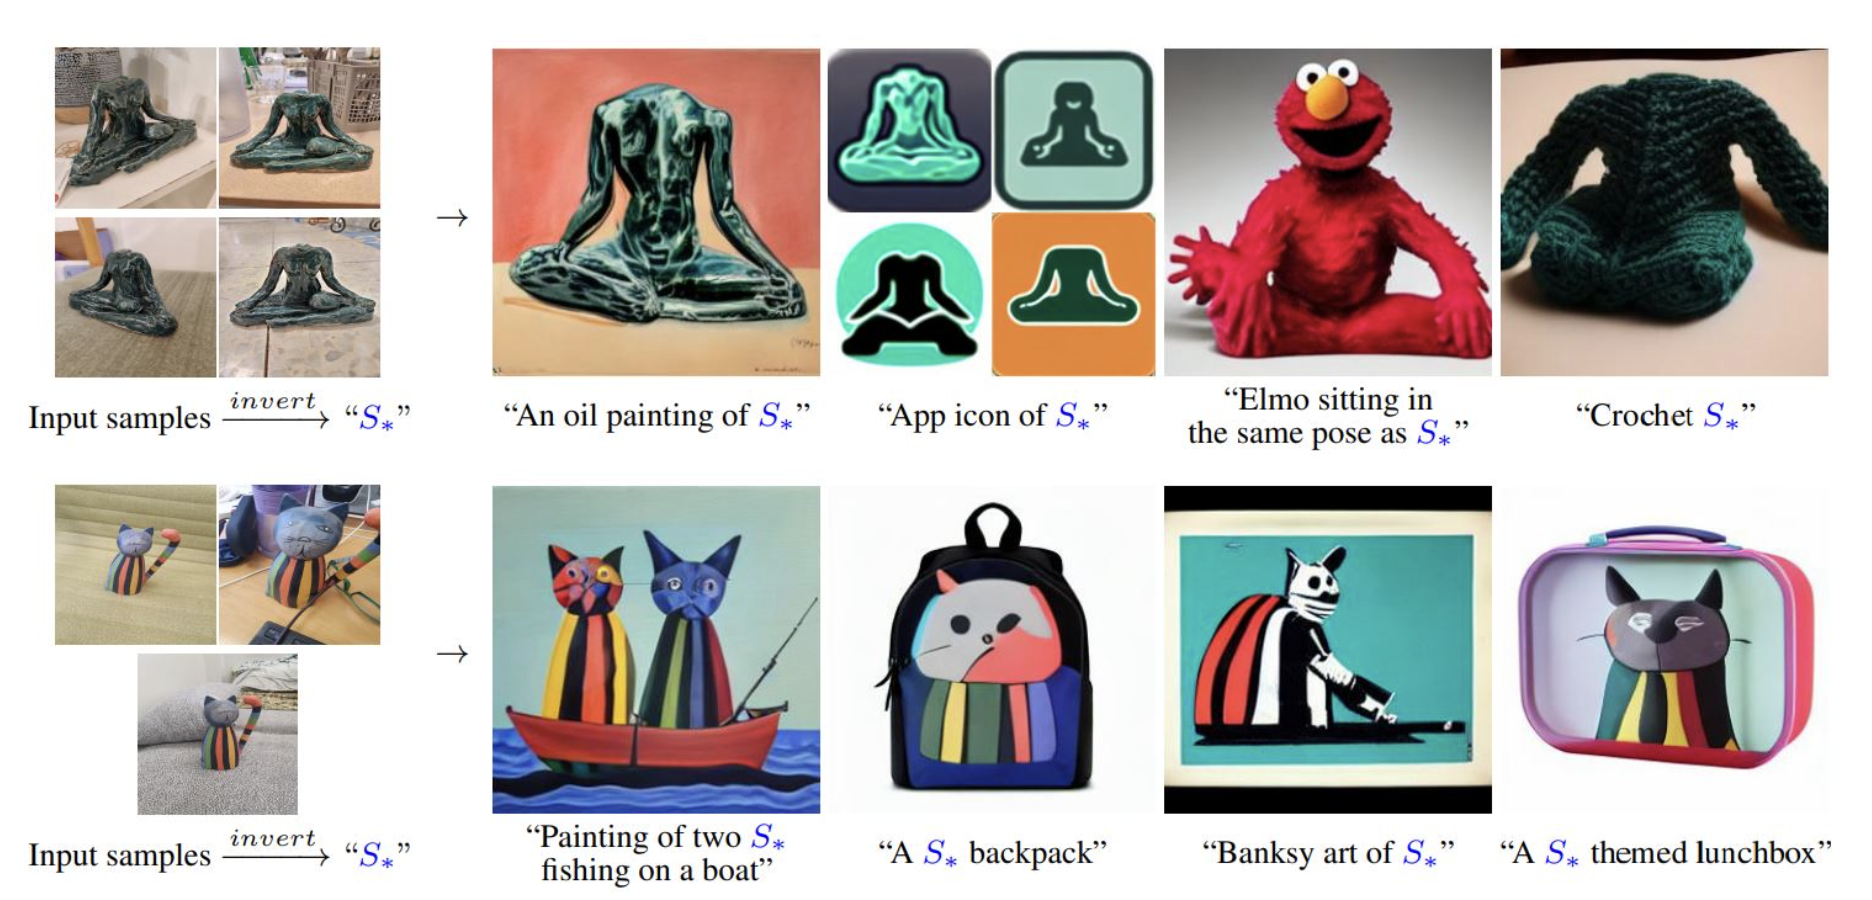
\includegraphics[width=\textwidth]{images/ti.png}
    \caption{Textual Inversion Results \cite{textualinversion2022}}
\end{figure}


\subsection{Full Model Training}
On the other side of the spectrum, full model training approaches such as Dreambooth push the boundaries by employing autogenous, class-specific prior preservation. This technique fine-tunes the entire model to adeptly generate images of a specific subject in various contexts, thereby broadening the model's versatility and adaptive capabilities \cite{dreambooth}. Similarly, Custom Diffusion updates the model by fine-tuning a selective set of weights, specifically targeting the key and value mappings in the cross-attention layers. This method underscores a targeted and efficient means of updating the model, ensuring that new concepts are seamlessly woven into the model's fabric without extensive retraining \cite{customDiffusion}. Furthermore, SINE reimagines model modification through classifier-free guidance (CFG) adjustments, enhancing the model's fidelity to desired outputs in the absence of explicit class labels, thus offering a robust and flexible framework for concept introduction \cite{sine}. Lastly, Break-A-Scene introduces a novel paradigm by enabling the learning of multiple concepts from a singular image, deviating from the conventional one-concept-per-multiple-images approach. This strategy showcases an efficient pathway to enrich the model's comprehension and creative scope \cite{breakAScene}. Through these full model training techniques, the landscape of generative modeling is witnessing a paradigm shift towards more dynamic, adaptive, and personalized image generation, promising a future where models can more accurately reflect the diversity and specificity of human imagination.




The convergence of these methodologies underlines a pivotal evolution in the development of diffusion models, marking a significant leap toward creating more adaptive, personalized, and context-aware generative models.









\begin{equation} \label{eq:1}
    \mathbb{E}_{x,c,e,\varepsilon,t} \left[ w_t \left\| \mathcal{X}_\theta (\alpha_t X + \sigma_t \varepsilon, c) - X \right\|^2 \right] 
    + \lambda w_t' \left\| \mathcal{X}_\theta (\alpha_t' X_{pr} + \sigma_t' \varepsilon', c_{pr}) - X_{pr} \right\|^2,
    \end{equation}



\begin{figure}[H]
    \centering
    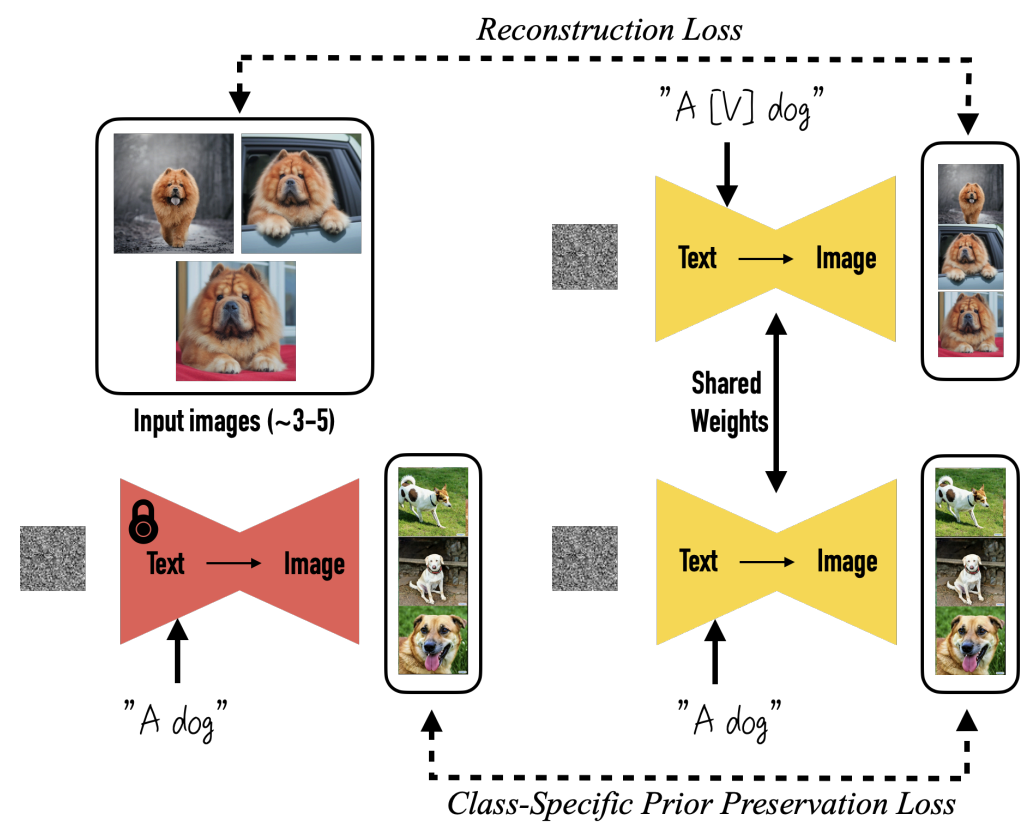
\includegraphics[width=0.55\textwidth]{images/dreambooth_training.png}
    \caption{Finetuning Dreambooth: Fine-tuning. Given $\sim 3-5$ images of a subject we finetune a text-to-image diffusion model with the input images paired
    with a text prompt containing a unique identifier and the name of
    the class the subject belongs to (e.g., "A [V] dog"), in parallel, we
    apply a class-specific prior preservation loss, which leverages the
    semantic prior that the model has on the class and encourages it to
    generate diverse instances belong to the subject's class using the class name in a text prompt (e.g., "A dog"). \cite*{dreambooth}}
\end{figure}
    

\begin{figure}[H]
    \centering
    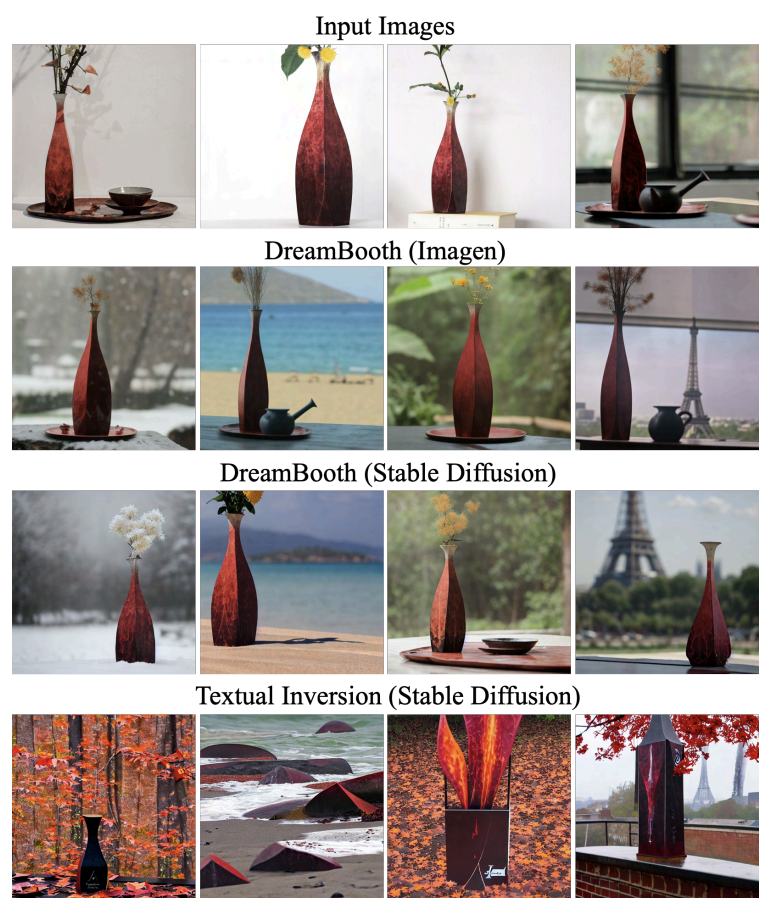
\includegraphics[width=0.4\textwidth]{images/dreambooth_ti_comp.png}
    \caption{Comparisons with Textual Inversion [20] Given 4
    input images (top row), we compare: DreamBooth Imagen (2nd
    row), DreamBooth Stable Diffusion (3rd row), Textual Inversion
    (bottom row). Output images were created with the following
    prompts (left to right): “a [V] vase in the snow”, “a [V] vase on
    the beach”, “a [V] vase in the jungle”, “a [V] vase with the Eiffel
    Tower in the background”. DreamBooth is stronger in both subject
    and prompt fidelity. \cite*{dreambooth}}
\end{figure}

\begin{table}[h!]
    \centering
    \begin{tabular}{ | m{5em} | m{5cm}| m{8cm} | m{2cm} | }
    \hline
    \textbf{Name} & \textbf{Tags} & \textbf{Text} & \textbf{Citations} \\
    \hline
    Textual Inversion & Embeddings & Learns textual embedding for new concept &  \\
    \hline
    Dreambooth & Full model \newline new loss & Trains full model using autogenous, class-specific prior preservation loss & \cite*{dreambooth}  \\
    \hline
    Custom Diffusion & Learns Attention KV & A small subset of model weights, namely the key and value mapping from text to latent features in the cross-attention layers. Fine-tuning these is sufficient to update the model with the new concept & \cite{customDiffusion} \\
    \hline
    ReVersion: & Embeddings & Learns embedding to learn relation instead of feature of image & \cite{reVersion} \\
    \hline
    SINE & Modifies CFG & Model-based classifier-free guidance & \cite{sine}\\
    \hline
    Break-A-Scene & Learning multiple concept & Learning multiple concepts using single image instead of learning one concept using multiple images & \\
    \hline
    \end{tabular}
    \caption{Contribution of different concept learning methods}
\end{table}
    

\section{Removing Concept}
The endeavor to remove specific concepts from diffusion models highlights a critical and multifaceted challenge in the realm of generative artificial intelligence, merging technical sophistication with ethical considerations. As these models increasingly permeate various sectors, the generation of undesired or controversial content raises significant concerns, necessitating interventions that are not only technologically adept but also cognizant of broader societal implications and individual privacy concerns. This complex interplay demands solutions that adeptly navigate the technical intricacies of altering model outputs without compromising on accuracy or creativity, while also ensuring adherence to ethical standards, legal requirements, and cultural sensitivities. As such, the pursuit of concept removal from diffusion models transcends mere algorithmic adjustments, embodying a broader commitment to responsible AI development that respects human values and rights, thereby reinforcing the importance of aligning technological advancements with ethical imperatives in the development and deployment of generative models.

\subsection{Dataset Curation and Post-Hoc Modifications}
Methods to mitigate undesirable image generation have primarily followed two paths. The first approach involves censoring or selectively curating the training dataset to exclude specific classes of images that are considered undesirable, such as removing all images of people or more narrowly targeting specific undesired content \cite{25,39,27,33}. While straightforward, this method is notably resource-intensive due to the significant computational demands of retraining large models. Furthermore, it risks unintended consequences stemming from large-scale censorship \cite{26}.

The alternative, post-hoc strategy modifies the output after training. This can be achieved through the use of classifiers to filter out undesired content \cite{3,21,29} or by incorporating guidance into the inference process \cite{38}. Although these methods are more cost-efficient and quicker to implement, they suffer from vulnerability; knowledgeable users can bypass these safeguards by manipulating model parameters \cite{43}.

In light of these limitations, recent developments have seen the emergence of novel techniques. For example, Stable Diffusion 2.0 represents an effort to retrain models on censored datasets \cite{30}, while Safe Latent Diffusion introduces state-of-the-art guidance-based approaches \cite{38}. Our investigation builds upon these foundations, proposing a third methodology that refines model parameters through a guidance-based model-editing technique, offering both rapid deployment and resilience against circumvention efforts.

\subsection{Image Cloaking}
Image cloaking emerges as a proactive measure enabling content creators to shield their works from being learned by generative models. By introducing adversarial perturbations, artists can obscure their images, effectively disguising them from machine learning algorithms either during training or inference, without impacting human perception significantly \cite{36,42}. This approach, however, diverges from the primary concern of concept removal from the perspective of model creators.

\subsection{Model Editing}
As an extension of concept removal, model editing seeks to adjust the generative capabilities of models without extensive retraining. Techniques vary from modifying specific neurons or layers \cite{7,23} to employing hypernetworks \cite{8,24} for text generators, and analogous methods for image synthesis, such as using textual or sketch inputs, gestures, or direct editing of features \cite{2,14,46,47}. The evolution towards model editing underscores the industry's shift towards more efficient and nuanced control over generative models, aligning with our proposed method of parameter tuning for concept removal.
Among these advancements, the "Forget-Me-Not" \cite*{zhang2023forgetmenot} approach represents a significant stride, utilizing a guidance-based model-editing technique that refines model parameters to selectively forget or correct specific concepts. This method enhances the flexibility and efficiency of concept manipulation in diffusion models, offering a solution that is both quick to deploy and robust against attempts to circumvent concept removal safeguards. The evolution towards model editing, as exemplified by "Forget-Me-Not," underscores the industry's shift towards more efficient and nuanced control over generative models, aligning with our proposed method of parameter tuning for concept removal.



\begin{table}[h]
    \centering
    \label{my-label}
    \begin{tabular}{|l|c|c|c|c|}
    \hline
    \textbf{Methods}      & \textbf{Performance}                     & \textbf{Integrity}                            & \textbf{Generality}                        & \textbf{Flexibility}                 \\ \hline
    Token Blacklisting    & \textcolor{red}{No forgetting}           & \textcolor{yellow}{Inevitably affects}                            & \textcolor{yellow}{Within the}                                 & \textcolor{yellow}{Tokenizer required}                    \\
                          &                                          & \textcolor{yellow}{other concepts}                              & \textcolor{yellow}{vocabulary of the}                        &                                       \\
                          &                                          & \textcolor{yellow}{sharing overlapping}                        & \textcolor{yellow}{tokenizer}                                 &                                       \\
                          &                                          & \textcolor{yellow}{prompts}                                      &                                           &                                       \\ \hline
    Naive Finetuning      & \textcolor{green}{Successfully}          & \textcolor{red}{Removes unrelated}           & \textcolor{green}{Applies to any}          & \textcolor{green}{Applies to any}     \\
                          & \textcolor{green}{removes concept}       & \textcolor{red}{concept by fault}            & \textcolor{green}{concepts with}           & \textcolor{green}{models}             \\
                          &                                          &                                               & \textcolor{green}{sufficient data.}        &                                       \\ \hline
    Forget-Me-Not         & \textcolor{green}{Successfully}          & \textcolor{green}{Maintains most of}                             & \textcolor{green}{Applies to any}                             & \textcolor{yellow}{Only applies to}                       \\
                          & \textcolor{green}{removes concept}       & \textcolor{green}{the model's}                                   & \textcolor{green}{concepts with few }                         & \textcolor{yellow}{models with cross}                     \\
                          &                                          & \textcolor{green}{integraity.}               & \textcolor{green}{data samples}                               & \textcolor{yellow}{attention}            \\ \hline
    \end{tabular}
    \caption{This table compares pros (green) and cons (red) on the four major aspects of concept forgetting between baselines and the proposed Forget-Me-Not. If an approach can handle an aspect to some extent, the corresponding explanation is marked in yellow. \cite*{zhang2023forgetmenot}}
    \end{table}
    

\begin{figure}[H]
    \centering
    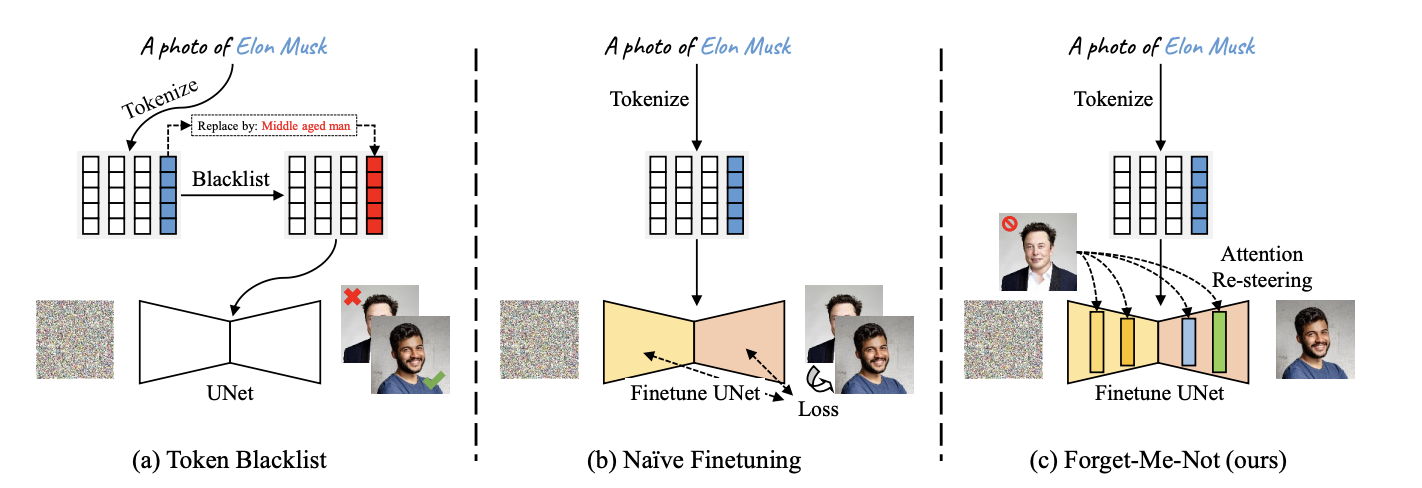
\includegraphics[width=1\textwidth]{images/concept_removal_comp.png}
    \caption{ This figure shows two baseline forgetting methods and our proposed Forget-Me-Not. The target concept to forget is Elon Musk.
    One baseline is (a) Token Blacklist that simply replaces the target token with a different one. The other baseline is (b) Naive Fintuning in
    which instead of replacing tokens, it finetunes model weights so that the new weights generate outputs containing unrelated concepts. Our
    method (c) Forget-Me-Not utilizes Attention Re-steering in which we finetune only UNet to minimize each of the intermediate attention
    maps associated with the target concepts to forget. \cite*{zhang2023forgetmenot}}
\end{figure}




\section{Applications}
In the rapidly evolving landscape of artificial intelligence, diffusion models have emerged as a groundbreaking approach, offering transformative capabilities across a wide array of applications. These models, through a process of iterative refinement, have unlocked unprecedented potential in creative and analytical tasks alike. Among their most notable applications are Text to Image generation, where models synthesize visually compelling images from descriptive text, blending creativity with precision to bridge the gap between textual concepts and their visual representations. In Image to Image translation, they adeptly modify or transform one image into another style or context, showcasing their versatility in reimagining visual content. Image editing with diffusion models goes a step further, allowing for nuanced adjustments and enhancements that redefine the boundaries of digital artistry. In the realm of Video, these models extend their prowess to dynamic sequences, enabling the generation and modification of video content with an eye for detail and continuity. The exploration into 3D brings a spatial dimension to their capabilities, where diffusion models generate and manipulate three-dimensional objects and environments, opening new frontiers in virtual and augmented reality. Lastly, their application in Document Layout emphasizes their utility beyond the visual arts, automating the design of document structures in a way that balances aesthetics with information delivery. This diverse spectrum of applications not only highlights the versatility of diffusion models but also sets the stage for their future developments, promising to redefine the intersection of technology and creativity.

\subsection{Text to Image}
Diffusion models have demonstrated remarkable achievements in the domain of text-to-image synthesis, showcasing their ability to creatively merge distinct concepts such as objects, shapes, and textures, thereby producing innovative imagery. This assertion was validated through the application of Stable Diffusion \cite{rombach2022highresolution} for crafting images from diverse textual descriptions, as illustrated in Figure 2.

The Imagen model, introduced by Saharia et al. \cite{saharia2022photorealistic}, represents a method for text-to-image synthesis, incorporating a text encoder and a series of diffusion models for crafting high-resolution images, conditioned on text embeddings produced by the encoder. Additionally, a novel benchmark for text-to-image evaluation named DrawBench was proposed. In terms of architecture, the authors developed Efficient U-Net to enhance efficiency, applying this design within their text-to-image synthesis experiments.

Gu et al. \cite{gu2022vector} put forward the VQ-Diffusion model, a novel approach for text-to-image synthesis that eliminates the unidirectional bias found in earlier methods. Through its unique masking strategy, it prevents error accumulation during inference. The model operates in two phases: initially utilizing a VQ-VAE to represent images as discrete tokens, followed by a discrete diffusion model acting on the VQ-VAE's latent space, guided by caption embeddings. This process is inspired by masked language modeling, replacing some tokens with a [mask] token.

Avrahami et al. \cite{avrahami2022blended} developed a text-conditional diffusion model reliant on CLIP \cite{radford2021learning} embeddings for both image and text. Employing a dual-stage approach, the first generates the image embedding, while the second, acting as a decoder, synthesizes the final image based on both the image embedding and the text caption. To create image embeddings, a diffusion model in the latent space was utilized, with a subjective human evaluation assessing the generative outcomes.

Addressing the slow sampling issue inherent in diffusion models, Zhang et al. \cite{zhang2022fast} introduced a novel discretization strategy that minimizes error and allows for larger step sizes, thereby reducing the number of required sampling steps. Utilizing high-order polynomial extrapolations for the score function and an Exponential Integrator to solve the reverse SDE, they significantly decreased the number of network evaluations needed without compromising the models' generative capabilities.

Shi et al. \cite{shi2022divae} merged a VQ-VAE \cite{oord2017neural} with a diffusion model for image generation. Initiating with the VQ-VAE for encoding, they substituted the decoder with a diffusion model, applying the U-Net architecture \cite{nichol2021improved} and incorporating image tokens into its mid-block.

Expanding on the concepts in Blattmann et al. \cite{blattmann2022retrieval}, Rombach et al. \cite{rombach2022textguided} introduced a modification for crafting artistic images by extracting nearest neighbors in the CLIP \cite{radford2021learning} latent space from a dataset, then guiding the reverse denoising process with these embeddings. Given the shared CLIP latent space for text and images, diffusion can also be text-guided. At inference, an artistic image database substitutes the original, steering the model to generate images reflective of the new dataset's style.

Jiang et al. \cite{jiang2022text2human} unveiled a framework to generate full-body human images with detailed clothing representation from three inputs: a human pose, and text descriptions for both the clothing's shape and texture. The initial phase encodes the shape description into an embedding vector, infusing it into a generative encoder-decoder module for shape mapping. Subsequently, a diffusion-based transformer leverages multiple texture-specific, multi-level codebooks for sampling the texture description's embedded representation, as suggested in VQ-VAE \cite{oord2017neural}. Initially, coarse-level codebook indices are sampled, with finer levels predicted via a feed-forward network, utilizing Sentence-BERT \cite{reimers2019sentencebert} for text encoding.



\subsection{Image To Image}
Saharia and colleagues \cite{Saharia2022Palette} introduce a unified framework for converting images across different contexts using diffusion models, concentrating on tasks such as colorization, inpainting, extension of image borders, and enhancement of compressed images. This framework remains consistent across these tasks, avoiding the necessity for individual modifications per task. They start by evaluating the effectiveness of L1 versus L2 losses, advocating for the latter due to its ability to increase the variety of generated samples. They also underscore the pivotal role of self-attention mechanisms in generating conditional images.

In an effort to facilitate image translation without corresponding pairs, Sasaki and team \cite{Sasaki2021UNITDDPM} develop a strategy that employs two diffusion models trained in tandem. Each model, through the process of reverse denoising, incorporates feedback from the other model's ongoing outputs. Additionally, they introduce a cycle-consistency loss to refine the training of these models.

Zhao et al. \cite{Zhao2022EGSDE} focus on enhancing the efficacy of image translation models based on diffusion by equally valuing source domain data. They use an energy-based approach that operates on both the source and target domains to guide the stochastic differential equation (SDE) solver. This method produces images that maintain universal features while accurately transferring domain-specific attributes. The model utilizes dual feature extractors, each tailored to a particular domain.

Wang and colleagues \cite{Wang2022Pretraining} leverage the pretrained GLIDE model to create a semantically rich latent space for image generation. By modifying the model's architecture to suit various conditions and then fine-tuning it for specific tasks, they achieve notable improvements. This process involves an initial focus on training a new encoder while keeping the decoder static, followed by concurrent training of both components. Adversarial training techniques and normalization strategies are also applied to further refine the quality of generated images.

Li et al. \cite{Li2022VQBB} propose a novel image translation diffusion model that combines the concepts of Brownian bridges and Generative Adversarial Networks (GANs). Their approach starts with encoding images via a Vector Quantized GAN, followed by a diffusion process that acts as a Brownian bridge in the quantized latent space, facilitating the transition between source and target domains. Subsequently, another VQ-GAN decodes these quantized representations to generate the translated image. Each GAN is trained independently within its respective domain.

Building on their previous research, Wolleb and associates \cite{Wolleb2022MultiTask} enhance their diffusion model by integrating a task-specific model in lieu of the standard classifier. This model enriches the sampling process by incorporating gradients from a network designed for a specific application, demonstrated through either a regression or segmentation task. This approach benefits from the existing diffusion model frameworks, eliminating the necessity for comprehensive retraining except for the component tailored to the specific task.


\subsection{Image editing}
Meng et al. \cite{Meng2021SDEdit} explored the application of diffusion models in tasks such as stroke painting, stroke-based editing, and image composition, starting with images that offer some form of guidance. These models preserve the original images' characteristics while smoothing out deformations through a forward diffusion process, and subsequently, a reverse process is applied to denoise these images to produce realistic outputs according to the provided guidance, effectively solving the reverse stochastic differential equation (SDE) without necessitating specialized datasets or modifications in training.

An earlier method for modifying specific image regions based on natural language descriptions was introduced \cite{avrahami2022blended}, where users define regions for editing via a mask. This approach uses CLIP guidance to generate images according to text inputs. However, it was observed that merging the generated output with the original image did not always result in a globally coherent image. To overcome this, a modified denoising process was applied that incorporates the masked latent image with a noisy version of the original image during each iteration.

Advancing this work, Avrahami et al. applied latent diffusion models for localized image editing through text. This method encodes both the image and a dynamically adjustable mask into the latent space, where a diffusion process guided by textual descriptions within the target area takes place \cite{Avrahami2022BlendedLatent}. Inspired by Blended Diffusion \cite{avrahami2022blended}, this technique uniquely combines the masked region in latent space with the contemporaneously noised image before decoding, resulting in enhanced performance and efficiency.



\subsection{Video}
In the exploration of video diffusion models, a broad spectrum of video analysis techniques is examined, encompassing the generation, modification, and interpretation of video content. These methods frequently adopt diffusion generation approaches or capitalize on the advanced generative capacities of diffusion models for subsequent applications. This survey prioritizes areas such as the creation of videos from text \cite{Singer2023MakeAV, Ho2022ImagenVH, Xing2023SimdaSA}, generating videos without predefined conditions \cite{Ho2022VideoDM, Hu2023LamdLV, Mei2023VidmVI}, and video modification guided by text descriptions \cite{Wu2023TuneAV, Esser2023StructureAC, Molad2023DreamixVD}, among others.

\subsection{Creation of Videos from Text}
Creation of Videos from Text is concerned with the automated transformation of textual narratives into videos. This requires the interpretation and conversion of text-described scenes, objects, and actions into a sequence of frames that visually cohere, thus yielding a video that is consistent both logically and visually. This technology finds application across various domains, including the automated production of films \cite{Zhu2023MoviefactoryAM}, animations \cite{He2023AnimateAS, Guo2023AnimatediffAY}, virtual reality, and educational materials \cite{Yang2023ProbabilisticAO}.

\subsection{Video Generation Without Predefined Conditions}
Video Generation Without Predefined Conditions describes the challenge of producing a continuous, visually coherent series of video frames from either stochastic noise or a predetermined starting point, with no reliance on specific input conditions. This mode of video generation distinguishes itself by not necessitating any external data or conditions \cite{Ho2022VideoDM, Hu2023LamdLV, Mei2023VidmVI}, thus challenging the generative model to independently learn the necessary temporal dynamics and visual elements for realistic and varied video content. This underscores the model's ability to understand content from unlabelled data and its potential for showcasing diversity.

\subsection{Text-driven Video Modification}
Text-driven Video Modification involves leveraging textual instructions to direct video content alterations. Through this method, a textual input specifies the desired video modifications, and the system employs this description to identify and implement changes based on the text-identified objects, actions, or scenes. This approach enhances editing efficiency and intuitiveness by enabling the use of natural language to describe edits \cite{Wu2023TuneAV, Esser2023StructureAC, Molad2023DreamixVD}, potentially diminishing the reliance on meticulous, frame-by-frame adjustments.

\subsection{3D}
The DreamFusion \cite*{poole2022dreamfusion} method represents a significant milestone in the field of artificial intelligence and computer vision, particularly in the synthesis of 3D models from textual descriptions. This innovative approach leverages a loss based on probability density distillation to utilize a pretrained 2D diffusion model as a prior for the optimization of a parametric image generator. Essentially, it optimizes a randomly-initialized Neural Radiance Field (NeRF) through a process akin to DeepDream, using gradient descent to ensure that the 3D model's 2D renderings from various angles align with the set low-loss criteria. This process enables the creation of 3D models that can be viewed from any angle, lit by any light source, and integrated into any 3D environment without the need for 3D training data or modifications to the existing diffusion model, showcasing the effectiveness of pretrained image diffusion models as priors.

The methodology behind DreamFusion involves initializing a NeRF-like model with random weights and iteratively refining it. This refinement process includes rendering views of the NeRF from random camera positions and angles, calculating a score distillation loss function that integrates with an existing image model like Imagen, and updating the NeRF parameters through an optimizer based on the computed gradients of the score distillation loss. This process is repeated for each text prompt, with each optimization cycle consisting of random sampling of camera and lighting conditions, rendering of the NeRF, and subsequent parameter updates. This iterative optimization results in the gradual refinement of the 3D model to more accurately reflect the textual description it is based on.

The compelling results of DreamFusion's process highlight the model's capability to produce detailed and realistic 3D renderings that closely match the given textual prompts. The provided images demonstrate the versatility of the model in generating a variety of scenes and objects, viewable from multiple perspectives. This underscores the model's potential in creating dynamic and interactive 3D models for a range of applications in 3D modeling, virtual reality, and more. DreamFusion's novel approach sets a new standard in the text-to-3D synthesis domain, offering a highly adaptable and efficient framework for the generation of intricate 3D models directly from text, thereby opening new avenues for both creative and practical applications in the field.








\subsection{Document Layout}
The paper LayoutDM \cite*{Inoue2023LayoutDM} by Naoto Inoue, Kotaro Kikuchi, Edgar Simo-Serra, Mayu Otani, and Kota Yamaguchi introduces a novel method for generating graphic layouts through a process named LayoutDM. This process leverages discrete state-space diffusion models, offering a significant advancement in controllable layout generation.

Graphic layouts are essential for visual communication, playing a pivotal role in various applications ranging from printed media to user interface design. The core challenge addressed by this work is the generation of plausible arrangements of elements within a layout, considering optional constraints such as the type or position of specific elements. Traditional methods often struggle with this task due to the structured nature of layout data, which necessitates careful consideration of the relationships between elements.

LayoutDM stands out by its use of discrete state-space diffusion models for layout generation. The model corrupts a layout in a modality-wise manner during the forward process and progressively denoises it, considering all elements and modalities in the reverse process. This approach naturally handles structured layout data in a discrete representation, learning to infer a noiseless layout from an initially corrupted input. Moreover, LayoutDM introduces a novel method to handle variable-length layout data by extending the discrete state space with a special PAD token, facilitating the incorporation of complex layout constraints through logit adjustment during inference.

The researchers demonstrate LayoutDM's superior performance over existing methods through extensive experiments on various layout generation tasks, utilizing large-scale datasets like Rico and PubLayNet. Their results showcase not only high-quality layout generation but also significant improvements over both task-specific and task-agnostic baselines.

A notable contribution of LayoutDM is its flexibility in conditional layout generation, addressing limitations of both autoregressive and non-autoregressive models. It enables the generation of variable-length elements without the need for additional training or external models, presenting a solution to the immutable dependency chain issue prevalent in autoregressive models. Through techniques such as masking and logit adjustment, LayoutDM effectively injects layout constraints during inference, demonstrating its ability to solve a wide range of tasks with a single model.

Furthermore, the paper explores various aspects crucial for effective layout generation, including modality-wise diffusion, adaptive quantization, and decoupled positional encoding. These innovations contribute to the model's ability to accurately capture and reproduce the structured and highly variable nature of layout data.

In summary, LayoutDM represents a significant step forward in the field of layout generation, providing a versatile and effective tool for synthesizing graphic layouts with optional constraints. Its approach combines the strengths of diffusion models with innovative techniques for handling structured and variable-length data, offering promising directions for future research in visual communication and design automation.


\section{Future research areas}
In recent years, diffusion models have made remarkable strides in the field of artificial intelligence, particularly in image, video, and 3D model generation. As outlined in the comprehensive survey, these models have evolved from theoretical concepts in thermodynamics to crucial tools in modern machine learning. While they have demonstrated impressive capabilities, there remains a vast scope for further advancement and refinement. The future research directions in this field are aimed at overcoming existing limitations and unlocking new possibilities, ensuring that diffusion models continue to evolve and remain at the forefront of technological innovation.

\subsection{Diverse Training Environments}
Exploring the integration of various data sources such as audio, video, and tactile feedback to enhance the training of diffusion models. This diversification can lead to more versatile models capable of handling a broader range of applications, including multimodal interaction and immersive virtual environments.
\subsection{Enhanced Latent Representations}
Investigating advanced techniques for improving the latent space representations of diffusion models. This includes developing methods for better interpretability, increased efficiency, and enhanced accuracy in handling complex data. Research in this area can significantly improve the models' ability to understand and generate more nuanced and contextually relevant content.
\subsection{Lower Computational Costs}
Focusing on developing more efficient algorithms and exploring novel hardware solutions to reduce the computational expense associated with training and operating diffusion models. This effort can make these models more accessible and sustainable, especially for applications requiring real-time processing or deployment in resource-constrained environments.
\subsection{Generating Finer Details}
Enhancing the capability of diffusion models to accurately generate fine details such as realistic text within images, correct anatomical features (like the correct number of fingers), and facial expressions. This requires advancements in both the models' understanding of intricate details and their ability to replicate these details accurately in the generated content.
\subsection{Ethical and Responsible AI}
As diffusion models become more powerful and widespread, it's crucial to address the ethical implications of their use. This includes developing guidelines and technologies for preventing misuse (such as deepfakes), ensuring privacy, and promoting fairness and inclusivity in the generated content.
\subsection{Interactivity and User Control}
Researching ways to enhance user interaction with diffusion models, allowing users to specify detailed preferences and control the generation process more precisely. This can include developing intuitive interfaces and control mechanisms that cater to both expert users and the general public.
\subsection{Integration with Other AI Technologies}
Exploring how diffusion models can be effectively combined with other AI technologies like reinforcement learning, symbolic AI, or decision-making algorithms to create more comprehensive AI systems capable of complex tasks like automated storytelling, content creation, or advanced simulations.
\subsection{Domain-Specific Applications}
Investigating the application of diffusion models in specific domains such as healthcare, education, and environmental modeling. This involves customizing the models to handle domain-specific data and requirements, potentially leading to breakthroughs in these fields.



\section{Conclusion}
In this comprehensive survey, we traversed the expansive and dynamic terrain of diffusion models, from their theoretical underpinnings in thermodynamics to their revolutionary applications in artificial intelligence, specifically in the domains of image, video, 3D model generation, and beyond. The journey through the evolution of diffusion models revealed their profound impact on the field of machine learning, showcasing their ability to generate high-quality, diverse outputs that push the boundaries of creativity and realism.

Throughout this exploration, we encountered the pivotal advancements that have cemented diffusion models as a cornerstone of modern generative AI. From the early implementations in image synthesis to the intricate mechanisms enabling text-to-image translations, each development has contributed to the models' increasing sophistication and versatility. We delved into the challenges that accompany diffusion models, such as computational efficiency and alignment with complex text prompts, and highlighted the innovative solutions proposed by the research community to address these issues.

The application of diffusion models extends beyond mere content creation; they have proven instrumental in editing, translating, and even removing content, demonstrating an unparalleled flexibility. This versatility, coupled with the continuous advancements in model architecture and training methodologies, signals a future where diffusion models could offer even more personalized, efficient, and ethically conscious solutions to a wide array of challenges in AI and beyond.

As we look to the horizon, the potential of diffusion models appears boundless. The ongoing research into enhancing their efficiency, accuracy, and ethical considerations paints a promising picture for the future. By continuing to refine and expand upon the capabilities of diffusion models, we can anticipate a new era of AI-driven creativity and innovation, where the boundary between human and machine-generated content blurs, leading to unprecedented opportunities for artistic expression, technological advancement, and societal impact.

In conclusion, this survey underscores the significant strides made in the development of diffusion models and their applications. It highlights the model's transformative potential across various domains, advocating for continued exploration and innovation to unlock even greater capabilities. The journey of diffusion models is far from complete; it is a field ripe with opportunities for discovery, improvement, and revolutionary applications that will continue to shape the future of artificial intelligence.


\section*{References}

\printbibliography[heading=none]


\end{document}
